% arguelles v2.3.0
% author: Michele Piazzai
% contact: michele.piazzai@uc3m.es
% license: MIT

% Copied from GitHub: https://github.com/piazzai/arguelles

\documentclass[compress,12pt]{beamer}

\usetheme{Arguelles}

\title{AIICP}
\subtitle{Artificial Intelligence Image Correction Pipeline}
\event{}
\date{}
\author{Nilton Aguiar dos Santos}
% \institute{University of \TeX}
% \email{name@domain.com}
% \homepage{www.mywebsite.com}
% \github{username}

\begin{document}

\frame[plain]{\titlepage}

\section{Síntese de Imagem Artificial}

\begin{frame}{Stable Diffusion}
    \textit{Stable Diffusion} é um modelo que gera imagens a partir de texto. Ele funciona comprimindo a imagem em um espaço latente de baixa dimensão e depois reconstruindo-a.
	
    O espaço latente é um vetor numérico que representa as características essenciais da imagem. O processo consiste em adicionar e remover ruído da imagem de forma controlada baseado no espaço semântico.
\end{frame}

\section{Princípios da \textit{Pixel Art}}

\begin{frame}{Definição}
	\begin{columns}
		\begin{column}{0.5\textwidth}
                A \textit{pixel art} é uma forma de arte digital na qual as imagens são construídas utilizando \textit{pixels} como seu bloco de construção. Associada com gráficos de baixa resolução da era computacional de 8 e 16-bit.
		\end{column}
		\begin{column}{0.5\textwidth}  %%<--- here
			\begin{center}
                {\textit{Pixel Art} Produzida por Humano.} 
				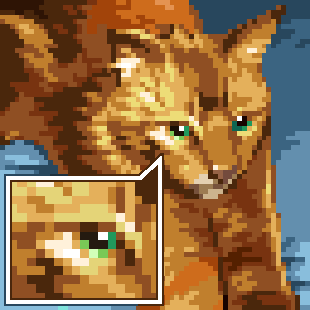
\includegraphics[width=0.85\textwidth]{Images/catImage.png}
			\end{center}
		\end{column}
	\end{columns}
\end{frame}

\begin{frame}{Papel Individual}
	\begin{columns}
		\begin{column}{0.5\textwidth}
                Uma das principais restrições na construção da arte que possibilita que ela se assemelhe com um arte \textit{pixel} é no papel individual de cada \textit{pixel} mostrado na imagem.
                \vfill
                Na qual é possível alterar todo o significado da arte modificando somente alguns \textit{pixels}.
			        
		\end{column}
		\begin{column}{0.5\textwidth}  %%<--- here
			\begin{center}
                {\textit{Pixel Art} Produzida por Humano.} 
				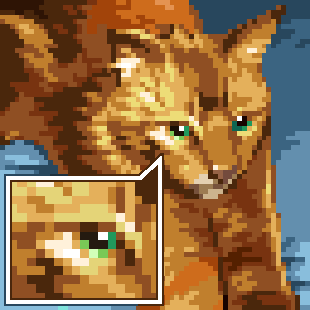
\includegraphics[width=0.85\textwidth]{Images/catImage.png}
			\end{center}
		\end{column}
	\end{columns}
\end{frame}


\begin{frame}{Colorização}
	\begin{columns}
		\begin{column}{0.5\textwidth}
			        
			{Outra característica comum na arte pixel é da baixa quantidade de cores disponíveis, originando-se da limitação gráfica que existia no inicio dos computadores. Onde a quantidade de cores se limitava em 8, 16 ou 32 dependendo da plataforma.}
            \vfill      
			{Como vemos no exemplo onde a imagem só contém 12 cores.}
			        
		\end{column}
		\begin{column}{0.5\textwidth}  %%<--- here
			\begin{center}
                {Pixel Art com 12bit de cores.} 
				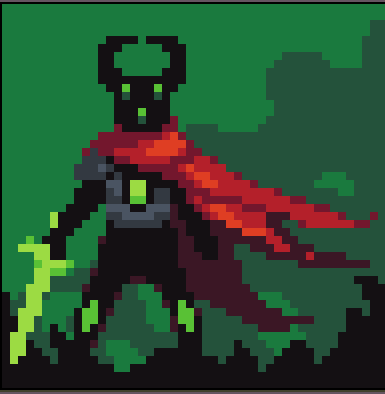
\includegraphics[width=0.85\textwidth]{Images/12bitImage.png}
			\end{center}
		\end{column}
	\end{columns}
\end{frame}

\begin{frame}{Colorização}
	\begin{columns}
		\begin{column}{0.5\textwidth}
			        
			{Outro exemplo é esta imagem na qual contém 16 cores.}
            \vfill
            {Podemos observar então que é importante a escolha de cada uma das cores a compor a imagem.}
			        
		\end{column}
		\begin{column}{0.5\textwidth}  %%<--- here
			\begin{center}
                {Pixel Art com 16bit de cores.}    
				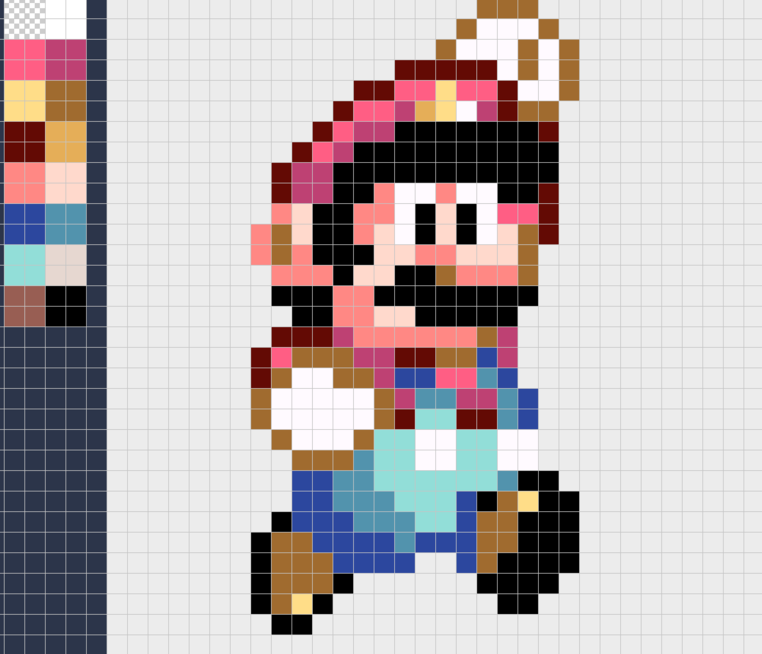
\includegraphics[width=0.85\textwidth]{Images/16bitImage.png}
			\end{center}
		\end{column}
	\end{columns}
\end{frame}

\section{Resultados Artificiais}

\begin{frame}{Situação Atual}
	\begin{columns}
		\begin{column}{0.5\textwidth}
                Com o advento da ferramenta de Difusão Estável para geração de imagens, houve a capacidade de geração de imagens em estilo de arte pixel. Porém falham nos princípios acima mencionados, como os exemplos a seguir:
                \vfill
                Imagem de uma paisagem no estilo \textit{Pixel Art}.
			        
		\end{column}
		\begin{column}{0.5\textwidth}  %%<--- here
			\begin{center}
                {Imagem gerada por IA.}    
				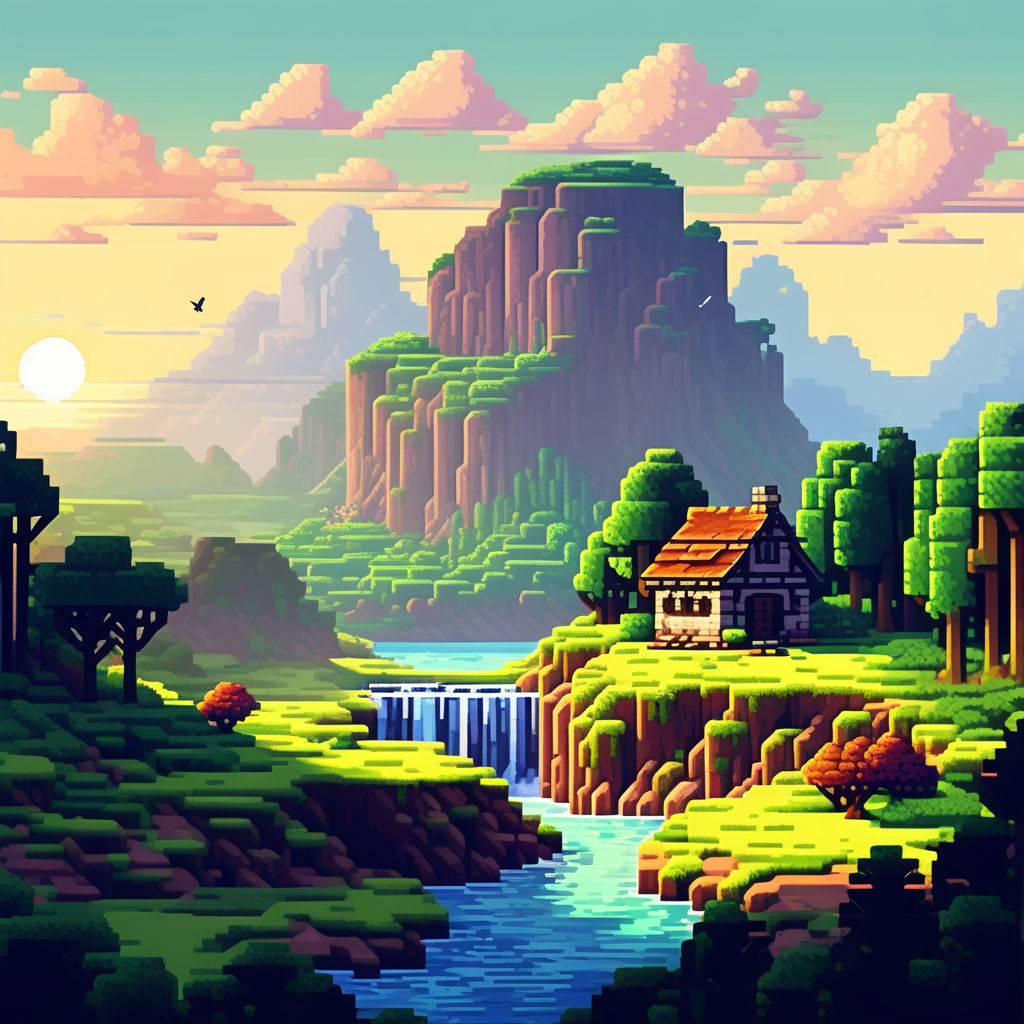
\includegraphics[width=0.85\textwidth]{Images/aiGeneratedPixelArt-1.jpeg}
			\end{center}
		\end{column}
	\end{columns}
\end{frame}

\begin{frame}{Identificação de falhas}
	\begin{columns}
		\begin{column}{0.5\textwidth}
                O resultado é satisfatório de primeira instância, porém ao observamos com um maior cuidado falhas surgem na própria fundamentação que determina o que é uma \textit{pixel art}, por exemplo:
            \begin{itemize}
                \item \textit{Pixels} com tamanhos variados
                \item Grande variação de cores
                \item Existência de curvas
                \item Existência de \textit{anti-aliasing}
            \end{itemize}
			        
		\end{column}
		\begin{column}{0.5\textwidth}  %%<--- here
			\begin{center}
                {Imagem gerada por IA.}    
				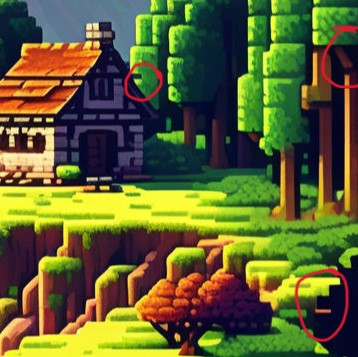
\includegraphics[width=0.85\textwidth]{Images/aiGeneratedPixelArt-1-P.jpeg}
			\end{center}
		\end{column}
	\end{columns}
\end{frame}

\begin{frame}{Persistência do problema}
	\begin{columns}
		\begin{column}{0.5\textwidth}  %%<--- here
			\begin{center}
                {Imagem gerada por IA.}    
				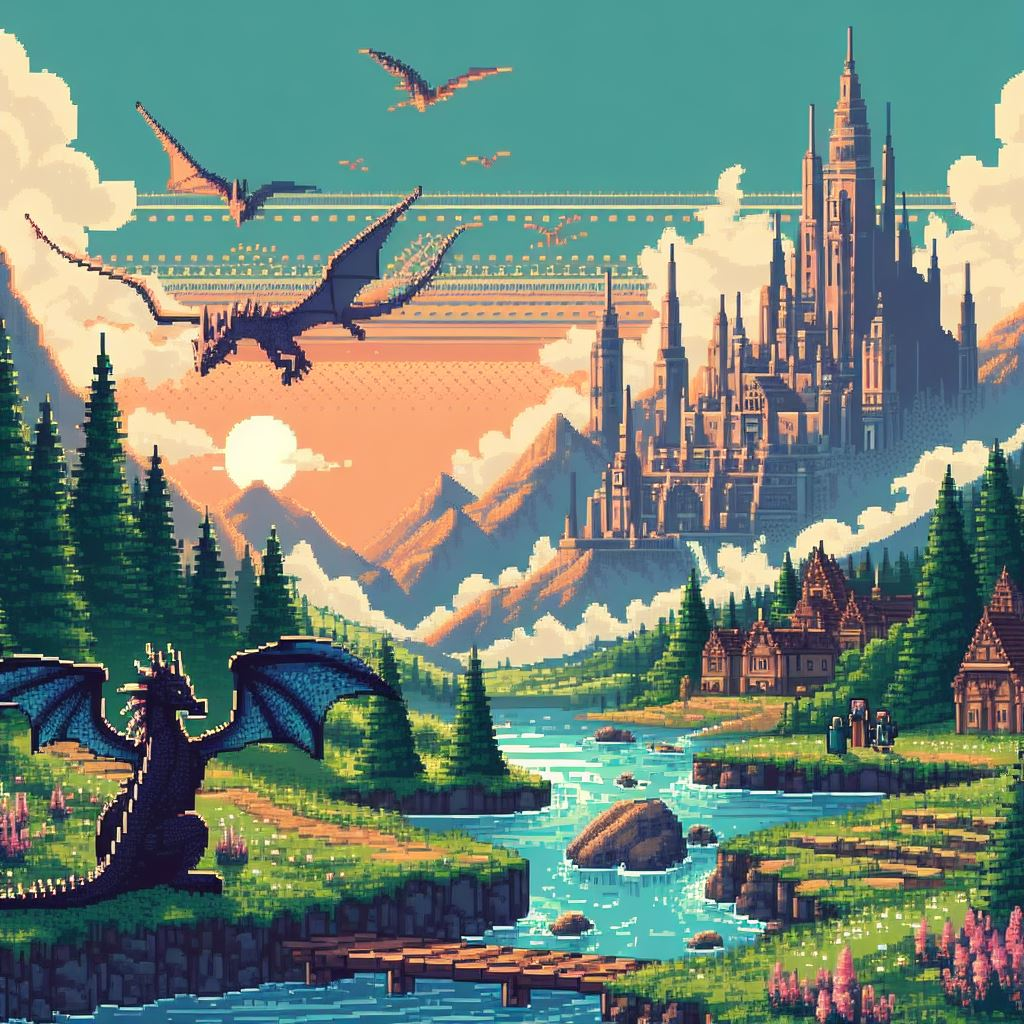
\includegraphics[width=0.85\textwidth]{Images/aiGeneratedPixelArt-2.jpg}
			\end{center}
		\end{column}
		\begin{column}{0.5\textwidth}  %%<--- here
			\begin{center}
                {Imagem gerada por IA.}    
				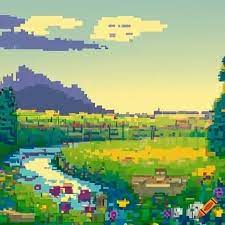
\includegraphics[width=0.85\textwidth]{Images/aiGeneratedPixelArt-3.jpg}
			\end{center}
		\end{column}
	\end{columns}
\end{frame}

\section{Solução}

\begin{frame}{Downscalling}
    O primeiro problema que encontramos é que há uma variação de tamanhos e formatos na imagem na qual retira o seu perfil artístico requerido. A solução é diminuir a resolução dela e após isso utilizar o método de Interpolação por Vizinho mais Próximo.
    
    Esse método preserva detalhes nítidos na arte, que é o que desejado.
\end{frame}

\begin{frame}{Donwscalling Resultados}
	\begin{columns}
		\begin{column}{0.5\textwidth}  %%<--- here
			\begin{center}
                {Não redimensionada.}
				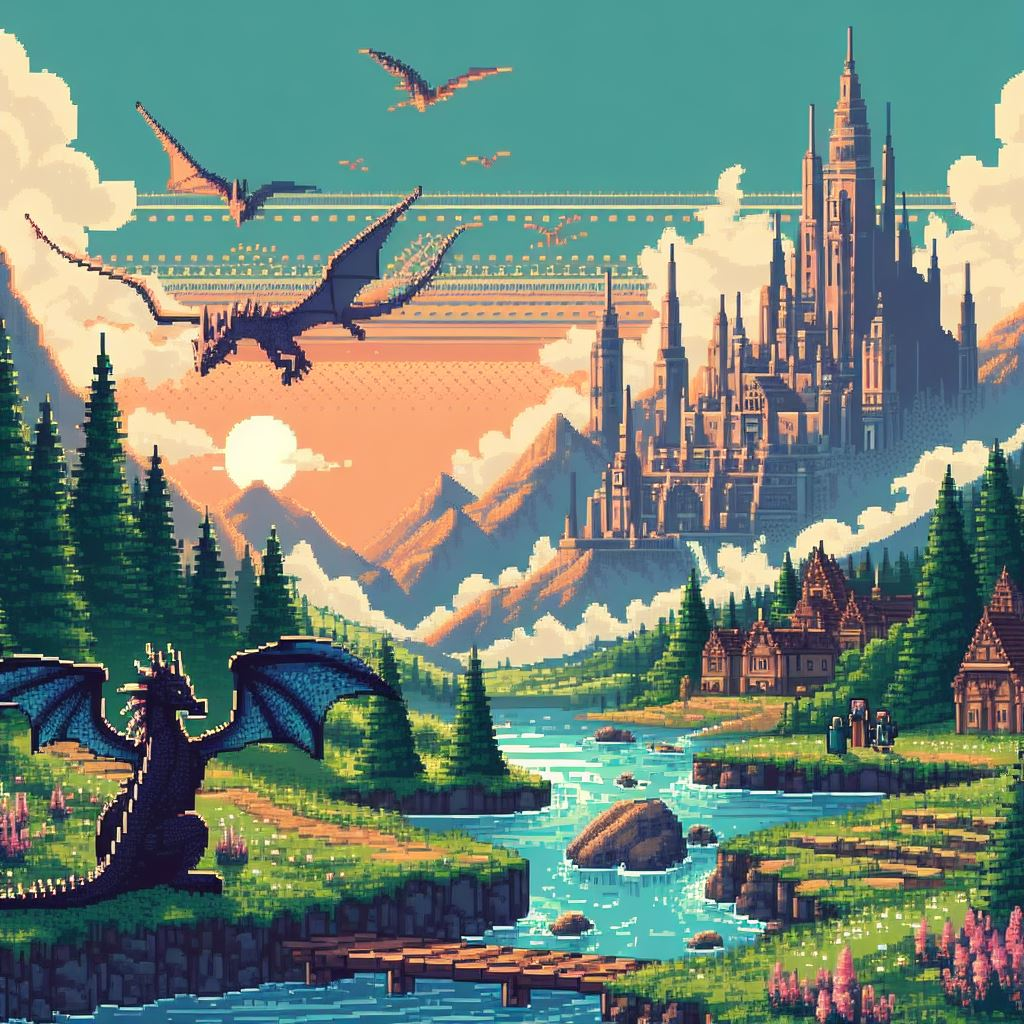
\includegraphics[width=0.85\textwidth]{Images/aiGeneratedPixelArt-2.jpg}
			\end{center}
		\end{column}
		\begin{column}{0.5\textwidth}  %%<--- here
			\begin{center}
                {Dimensionada.}
				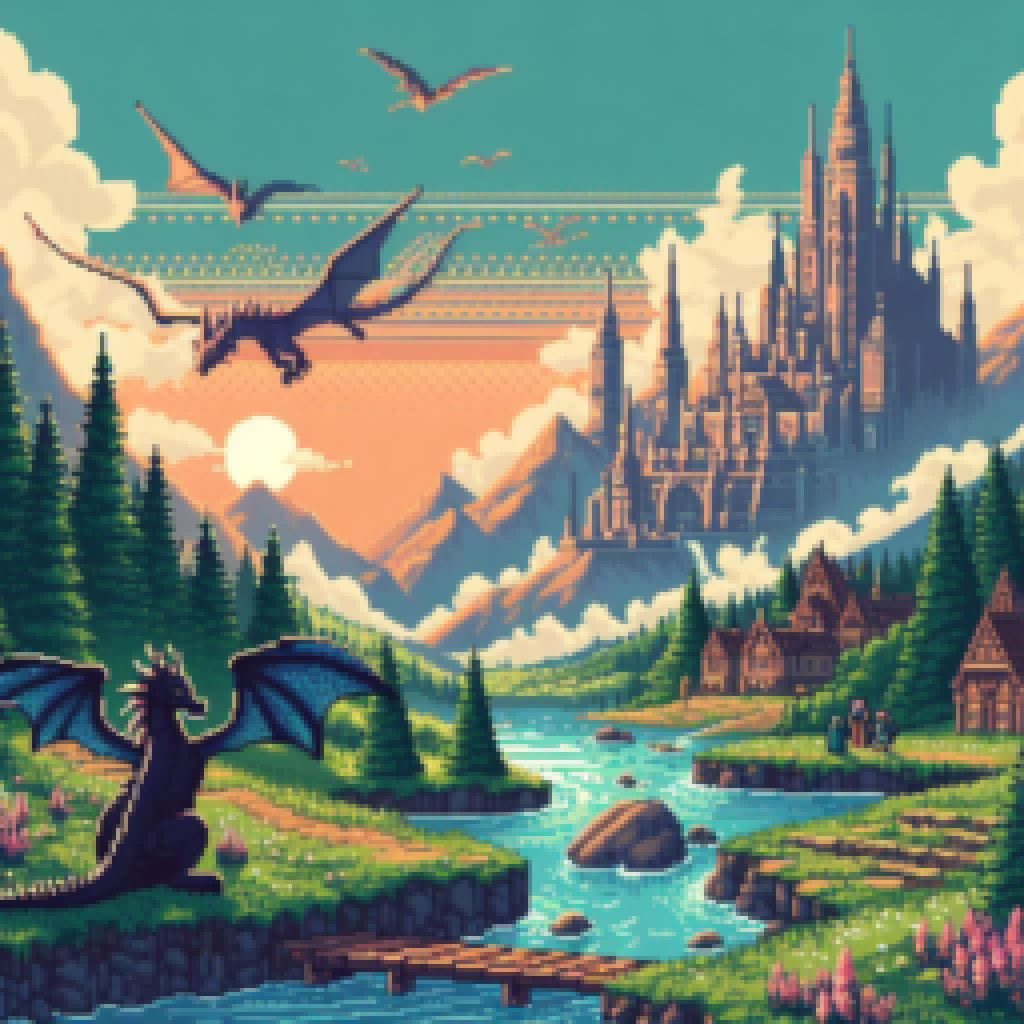
\includegraphics[width=0.85\textwidth]{Images/aiGeneratedPixelArt-2-T.png}
			\end{center}
		\end{column}
	\end{columns}
\end{frame}

\begin{frame}{Dithering}
    Não há muita evolução notável na aplicação somente dessa algoritmo, por isso é necessário seguir com mais um algoritmo.
    
    \textit{Dithering} é uma forma de barulho intencionalmente aplicado para evitar a ocorrência de padrões em larga escala. Existem várias funcionalidades para esse algoritmo mas um que deve ser mencionado é a utilização na transposição de uma imagem colorida em preto e branco de tal forma que as suas características principais perdurem.

    Porém nada impede que esse algoritmo explore não só dois bits, preto e branco, como qualquer numero de bits que for desejado. E o melhor a ser utilizado para a solução é o algoritmo de \textit{Dithering} de Bayer.     
\end{frame}
\begin{frame}[standout]
	\centering\large
    Discussão
\end{frame}
\end{document}
